%% =====================================================================
%%  Confidence-Guided Adaptive Reconstruction for Windowed QPE
%%  Target venue: MethodsX (Elsevier)
%%  Submission draft. Remaining \PLACEHOLDER markers are author-supplied
%%  fields only (affiliation, ORCID, repo URL, DOI, commit, funding).
%%  Build:  pdflatex main / bibtex main / pdflatex x2
%% =====================================================================
\documentclass[preprint,11pt]{elsarticle}

\usepackage{amsmath,amssymb,amsthm}
\usepackage{booktabs}
\usepackage{graphicx}
\usepackage{xcolor}
\usepackage{array}
\usepackage[hidelinks]{hyperref}
\usepackage{tikz}
\usetikzlibrary{arrows.meta,positioning,fit,backgrounds}
\usepackage[section]{placeins}
\usepackage{algorithm}
\usepackage{algpseudocode}

% ---- float placement: without these, the validation tables drift to the
% ---- end of the document, far from the text that discusses them.
\renewcommand{\topfraction}{0.9}
\renewcommand{\bottomfraction}{0.8}
\renewcommand{\textfraction}{0.07}
\renewcommand{\floatpagefraction}{0.7}
\setcounter{topnumber}{3}
\setcounter{bottomnumber}{2}
\setcounter{totalnumber}{5}

% ---- page efficiency (formatting only; no content is affected) -------
\setlength{\bibsep}{2pt plus 0.3ex}
\setlength{\textfloatsep}{10pt plus 2pt minus 2pt}
\setlength{\intextsep}{10pt plus 2pt minus 2pt}
\setlength{\abovedisplayskip}{6pt plus 2pt minus 2pt}
\setlength{\belowdisplayskip}{6pt plus 2pt minus 2pt}

% ---- draft markers: make every open item greppable and visible -------
\newcommand{\TODO}[1]{\textcolor{red}{\textbf{[TODO: #1]}}}
\newcommand{\PLACE}[1]{\textcolor{blue}{\textbf{[PLACEHOLDER: #1]}}}

% ---- evidentiary labels, carried over verbatim from the source notes -
\newcommand{\PROVEN}{\textsc{(proven)}}
\newcommand{\HEUR}{\textsc{(heuristic)}}
\newcommand{\EMPIR}{\textsc{(empirical)}}
\newcommand{\INVAR}{\textsc{(implementation invariant)}}

\newtheorem{proposition}{Proposition}
\newtheorem{lemma}{Lemma}
\newtheorem{corollary}{Corollary}
\newtheorem{invariant}{Invariant}

% Supplementary Information pointers (SI is a separate document, so these
% are literal rather than \ref, which cannot cross documents).
\newcommand{\SI}{Supplementary Information}
\newcommand{\SIaudit}{\SI{}~Sec.~S1}
\newcommand{\SItables}{\SI{}~Sec.~S2}
\newcommand{\SIartifacts}{\SI{}~Sec.~S3}

\newcommand{\Cw}{C_w}
\newcommand{\dcov}{\delta_{\mathrm{cov}}}
\newcommand{\Smax}{S_{\max}}
\newcommand{\beammax}{\texttt{beam\_max}}

\journal{Preprint}

\begin{document}

\begin{frontmatter}


\title{Where Windowed Shor's Algorithm Actually Fails, and What Fixing
It Buys: A Controlled Study}

\author[inst1]{Sanjay Lakshmanan R}
\ead{rajasanjay21@gmail.com}

\address[inst1]{Department of Computer Science and Engineering,
Amrita Vishwa Vidyapeetham, Chennai, India}

\begin{abstract}
Windowed quantum phase estimation makes Shor's algorithm cheaper in qubits
by splitting the phase register into narrow, independently measured windows
and reassembling the phase classically. What that costs, and where the
resulting pipeline actually breaks, has not been characterised. We report a
black-box characterisation of a from-scratch reproduction, followed by a
controlled evaluation of a fix.

The characterisation is the first half. Varying any single parameter in
isolation produces no failures at all across 435 trials --- a null result
with a specific cause, and a warning about one-factor-at-a-time designs in
this setting. Starving several classical budgets together on the same
instance fails 47.9\% of the time with no injected noise. Depolarising and
readout error compound super-additively, exceeding an independence baseline
in all nine cells of a factorial sweep. Direct fault injection leaves the
reconstruction logic intact under three of five conditions. A counterfactual
ladder applied to all 94 observed failures attributes 72\% of them to
classical budget starvation rather than to noise, corruption, or any defect
in the reconstruction logic. We also report a compilation cliff that caps
the reachable instance size before a shot is sampled, and an error of our
own: an audit script that reported a 55.4\% false-accept rate in the
carry-aware overlap check, which re-validation traced to a defect in the
audit rather than the mechanism, retracting a planned fix before it was
written.

The evaluation is the second half, of the confidence-guided reconstruction
method specified in the companion article. On a 144-cell grid the published
pipeline succeeds 52.1\% of the time and the full adaptive configuration
100\%; across three pre-registered held-out instances the combination
reaches 97.9--100\%. Matched-resource controls qualify this and are reported
as a primary finding: given each module's own realised budget spread
uniformly, no individual module is distinguishable from its control. The
evidence supports automatic, instance-adaptive selection of the
reconstruction budget, not a demonstrated superiority of confidence-guided
placement. All validation is noiseless, in simulation, and confined to
$N\in\{15,21\}$ by the measured compilation cliff.
\end{abstract}

\begin{keyword}
Shor's algorithm \sep quantum phase estimation \sep failure-mode analysis
\sep classical post-processing \sep ablation study \sep reproducibility
\end{keyword}

\end{frontmatter}

% =====================================================================
\section{Introduction}
\label{sec:intro}

Shor's algorithm \cite{shor1997} reduces factorisation to order-finding and
order-finding to quantum phase estimation
\cite{kitaev1995,cleve1998,nielsenchuang}. Textbook QPE needs a phase
register as wide as the requested precision. The windowed formulation
\cite{wqpe2025,modularshor2025} removes that requirement by partitioning the
register into narrow, independently measured, overlapping windows and
reassembling the full-precision phase classically. The qubit saving is real
and it is bought with classical work: reconstruction must recover one phase
from $W$ partial, individually ambiguous measurements.

That trade has been proposed and its correctness demonstrated. What has not
been established is where the resulting pipeline fails, how often, and
\emph{why} --- which is the question a practitioner deciding whether to
adopt it actually has. This article answers it in two halves, and the two
halves are methodologically different: the first is exploratory
characterisation of a system we did not design the failure modes of, the
second is a pre-registered controlled evaluation of a specific intervention.

\paragraph{Part I} characterises a from-scratch reproduction as a black box.
It reports a null result that matters (single-parameter sweeps find nothing),
the combined-stress regime where the pipeline does fail, a noise interaction
study, direct fault injection into the classical stage, a compilation cliff
that bounds every experiment in this article, and a counterfactual
attribution of all 94 observed failures. It also reports an error of our
own, and what re-validating it cost and saved.

\paragraph{Part II} evaluates the confidence-guided adaptive reconstruction
method specified in the companion article~\cite{methodpaper}, which replaces
the three fixed classical budgets with quantities computed from the measured
counts. The evaluation is seed-paired, spans four instances, and includes
matched-resource controls that change the conclusion.

\paragraph{What the reader should take from this.} The headline number ---
$52.1\%$ to $100\%$ on the canonical grid --- is the least interesting result
here, because it compares against an unmodified baseline that was never given
the extra resources the adaptive rule spends. The matched-resource controls
of Sec.~\ref{sec:matched} are the finding we would ask a reader to carry
away, and they are partly negative. What the modules buy is not a better
placement of a given budget; it is not having to choose the budget in
advance.

% =====================================================================
\section{The pipeline under test}
\label{sec:pipeline}

\subsection{Windowed reconstruction and its three fixed budgets}

The published method \cite{wqpe2025,modularshor2025} replaces one
$\ell$-qubit phase register with $W$ overlapping windows of width
$\ell_w\ll\ell$, each measured independently by its own block-local QPE
circuit, and reassembles the phase from the per-window measurement counts in
three classical steps: generate the top-$k$ candidate bit patterns per
window, stitch compatible candidates across overlaps under a carry-aware
consistency check with a beam of width $P$, and recover the order by
continued fractions. Factor extraction follows from an even order $r$ via
$\gcd(a^{r/2}\pm1,N)$.

Three quantities in that stage --- the retained candidate count $k$, the beam
width $P$, and the per-window shot count $S_w$ --- are fixed at configuration
time and identical for every window of every instance. They are the subject
of both halves of this article: Part I establishes that they are the binding
constraint, and Part II evaluates replacing them.

\subsection{The reproduction, and what counts as success}

All results here are from an independent from-scratch reproduction, not from
the original authors' code. Throughout, a trial \emph{succeeds} only if it
recovers a correct non-trivial factor pair of $N$ end to end. This is a
deliberately unforgiving criterion: it does not credit a partially correct
phase, and it makes every reported rate directly comparable across the two
halves.

One consequence of it shapes Part I. At the small multiplicative orders our
compilation ceiling permits (Sec.~\ref{sec:cliff}), the continued-fraction
multiplier search is extremely forgiving --- theoretically under-resolved
configurations still recover the correct order. Any characterisation that
sweeps one parameter at a time will therefore find nothing, and
Sec.~\ref{sec:ofat} shows that it does.

% =====================================================================
\part*{Part I --- Characterisation}
\addcontentsline{toc}{part}{Part I --- Characterisation}

\section{Characterisation design}
\label{sec:chardesign}

The characterisation treats the reproduction as a black box and probes it
along five axes, in the order they were run: single-parameter sweeps
(Sec.~\ref{sec:ofat}), combined budget starvation
(Sec.~\ref{sec:combined}), injected noise (Sec.~\ref{sec:noise}), direct
fault injection into the classical stage (Sec.~\ref{sec:adversarial}), and
scaling (Sec.~\ref{sec:cliff}). A counterfactual attribution pass over every
failure any of them produced closes Part I (Sec.~\ref{sec:attribution}).

Each trial is seeded from its grid coordinates, and the simulator's sampling
is seeded from that, so any cell reproduces exactly on re-run. All raw
per-trial records are released.

\section{One factor at a time proves nothing here}
\label{sec:ofat}

We swept six parameters one at a time --- total precision (4--12), window
size (2--8), overlap (0--3), candidate count (1--16), beam width (1--4096),
and shots (16--16384) --- holding the rest at their defaults, across three
small $(N,a)$ pairs, 15 trials per parameter value.

\textbf{Every one of the 435 trials succeeded.} Table~\ref{tab:ofat}
reports the sweep; every cell is $15/15$, with a $95\%$ Wilson lower bound of
$0.796$. A factorial logistic regression of success on the three noise
levels (Fig.~\ref{fig:logistic}) likewise finds nothing: the largest
coefficient is two-qubit depolarising error at $-0.452$, and all three
confidence intervals cross zero.

This is a genuine null result with a specific cause rather than an absence of
evidence. At the orders reachable here the continued-fraction search absorbs
substantial phase error, so a configuration that is theoretically
under-resolved still recovers the right order. \textbf{The methodological
consequence is the point:} a one-factor-at-a-time design applied to this
pipeline will report that it has no failure modes, and be wrong. We report
the null in full because it is what motivated the design of
Sec.~\ref{sec:combined}, and because anyone characterising a comparable
pipeline is likely to start the same way.

\begin{table}[htbp]
\centering\small
\caption{Single-parameter sweep. Each row is one parameter value at 15
seed-paired trials with all other parameters at their defaults. Every cell
succeeded; the interval is a $95\%$ Wilson score interval, whose lower bound
of $0.796$ is what 15 successes out of 15 supports. From
\texttt{phase1\_ofat.csv}.}
\label{tab:ofat}
\begin{tabular}{@{}llrl@{}}
\toprule
Parameter & Values swept & Trials & Success \\
\midrule
Total precision $\ell$   & 4, 6, 8, 10, 12          & 75 & 15/15 each \\
Window size $\ell_w$     & 2, 3, 4, 6               & 60 & 15/15 each \\
Overlap $o$              & 0, 1, 2, 3               & 60 & 15/15 each \\
Candidate count $k$      & 1, 2, 4, 8, 16           & 75 & 15/15 each \\
Beam width $P$           & 1, 4, 16, 64, 256        & 75 & 15/15 each \\
Shots $S_w$              & 16, 64, 256, 1024, 4096, 16384 & 90 & 15/15 each \\
\midrule
\textbf{Total}           &                          & \textbf{435} & \textbf{435/435} \\
\bottomrule
\end{tabular}
\end{table}

\begin{figure}[htbp]
\centering
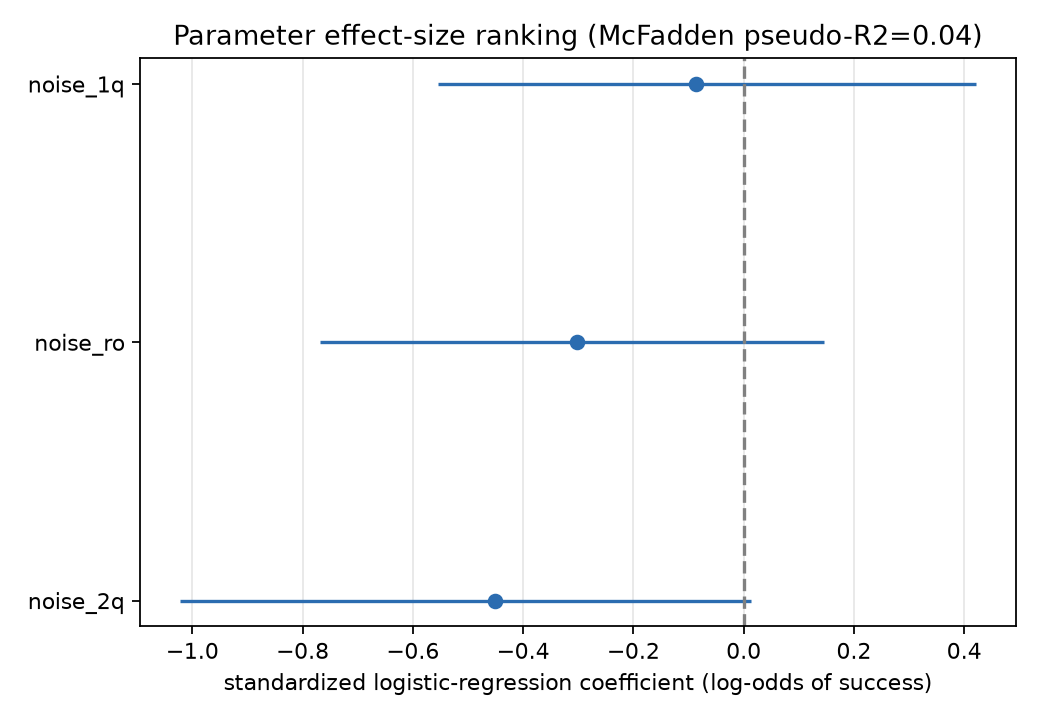
\includegraphics[width=0.78\linewidth]{../Data/failure_study/plots/logistic_effect_sizes.png}
\caption{\textbf{Standardised logistic-regression effect sizes for the three
noise channels.} Two-qubit depolarising error is the largest single driver
at $-0.452$, but all three intervals cross zero: at single-source levels, no
noise channel is individually distinguishable from none. The interaction
that does matter is in Sec.~\ref{sec:noise}. Rendered from
\texttt{phase1\_ofat.csv}.}
\label{fig:logistic}
\end{figure}

\section{Starving budgets together}
\label{sec:combined}

The same six parameters, constrained \emph{simultaneously}, tell the
opposite story. On $(N{=}21,a{=}19,r{=}6)$ we ran a 144-cell grid holding
$k\in\{1,2\}$, $P\in\{1,2\}$ and $S_w\in\{4,8,16\}$ while maximising
precision ($\ell\in\{16,24,32\}$) and sweeping overlap ($o\in\{0,3\}$).

\textbf{69 of 144 trials failed --- $47.9\%$ --- with zero injected noise and
zero corruption.} The same instance succeeds on every trial when any single
one of those budgets is relaxed. This grid is the canonical evaluation grid
for everything in Part II.

Two features of it are worth stating plainly. It is an adversarial regime,
deliberately chosen to make failures observable, and it is not
representative of a well-provisioned run. But it is also not artificial: each
constrained value lies inside the range a practitioner might reasonably pick
to save classical time, and nothing in the published method warns which
combinations are unsafe. The failure appears only in combination, which is
precisely why the sweep of Sec.~\ref{sec:ofat} could not find it.

\section{Noise compounds super-additively}
\label{sec:noise}

We injected depolarising error on one- and two-qubit gates and readout error,
first individually and then factorially. Individually, none of the three is
distinguishable from no noise at all, even at $30\%$ error
(Fig.~\ref{fig:logistic}).

Factorially they compound, and they compound \emph{more than independently}.
Table~\ref{tab:noise} crosses two-qubit and readout error at three levels
each. The observed success rate exceeds --- in the sense of falling below in
success, hence exceeding in damage --- the rate an independence assumption
would predict in \textbf{all nine cells}, by between $4.7$ and $9.9$
percentage points. The worst cell, both channels high, succeeds $81.5\%$ of
the time.

\begin{table}[htbp]
\centering\small
\caption{Factorial noise interaction, two-qubit depolarising against
readout error, 27 trials per cell. ``Independence'' is the success rate
predicted by treating the two channels as acting independently at their
measured single-source rates; ``excess'' is the shortfall of the observed
rate against it. Every cell is positive, so the channels compound
super-additively. From \texttt{phase2\_noise\_combined.csv}.}
\label{tab:noise}
\begin{tabular}{@{}llrrr@{}}
\toprule
2-qubit & Readout & Observed & Independence & Excess \\
\midrule
none & none & 0.963 & 0.892 & $+0.071$ \\
none & med  & 0.926 & 0.857 & $+0.069$ \\
none & high & 0.926 & 0.834 & $+0.092$ \\
med  & none & 1.000 & 0.904 & $+0.096$ \\
med  & med  & 0.926 & 0.868 & $+0.057$ \\
med  & high & 0.926 & 0.845 & $+0.081$ \\
high & none & 0.889 & 0.822 & $+0.067$ \\
high & med  & 0.889 & 0.790 & $+0.099$ \\
\textbf{high} & \textbf{high} & \textbf{0.815} & 0.768 & $+0.047$ \\
\bottomrule
\end{tabular}
\end{table}

\begin{figure}[htbp]
\centering
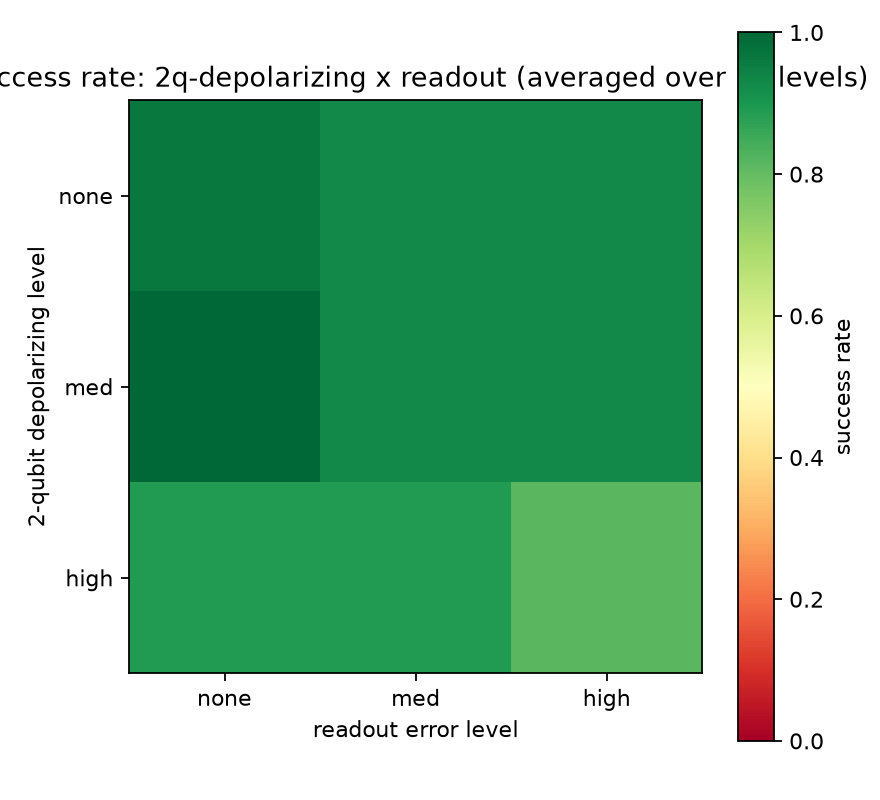
\includegraphics[width=0.72\linewidth]{../Data/failure_study/plots/noise_combined_heatmap.png}
\caption{\textbf{Success rate across the factorial noise grid.} The gradient
runs diagonally: neither channel alone moves the outcome much, and their
combination does. Rendered from \texttt{phase2\_noise\_combined.csv}.}
\label{fig:noise}
\end{figure}

\section{Direct fault injection into the classical stage}
\label{sec:adversarial}

Sweeps perturb inputs; this section perturbs the reconstruction stage
itself, injecting five conditions at 32 trials each
(Fig.~\ref{fig:adversarial}).

Three conditions leave the outcome untouched at $100\%$: a clean control, a
post-hoc bit flip, and the insertion of an incorrect high-weight candidate.
The stitching stage rejects or out-ranks all three. Removing the true
candidate from a window drops success to $78.1\%$ --- not to zero, because
overlap redundancy can still recover the phase from the remaining windows.
Corrupting an overlap region is the only severe condition, at $43.8\%$.

That last figure was originally attributed to the carry-aware consistency
check being over-permissive. Section~\ref{sec:retraction} reports why that
attribution was wrong, and what the correct one is.

\begin{figure}[htbp]
\centering
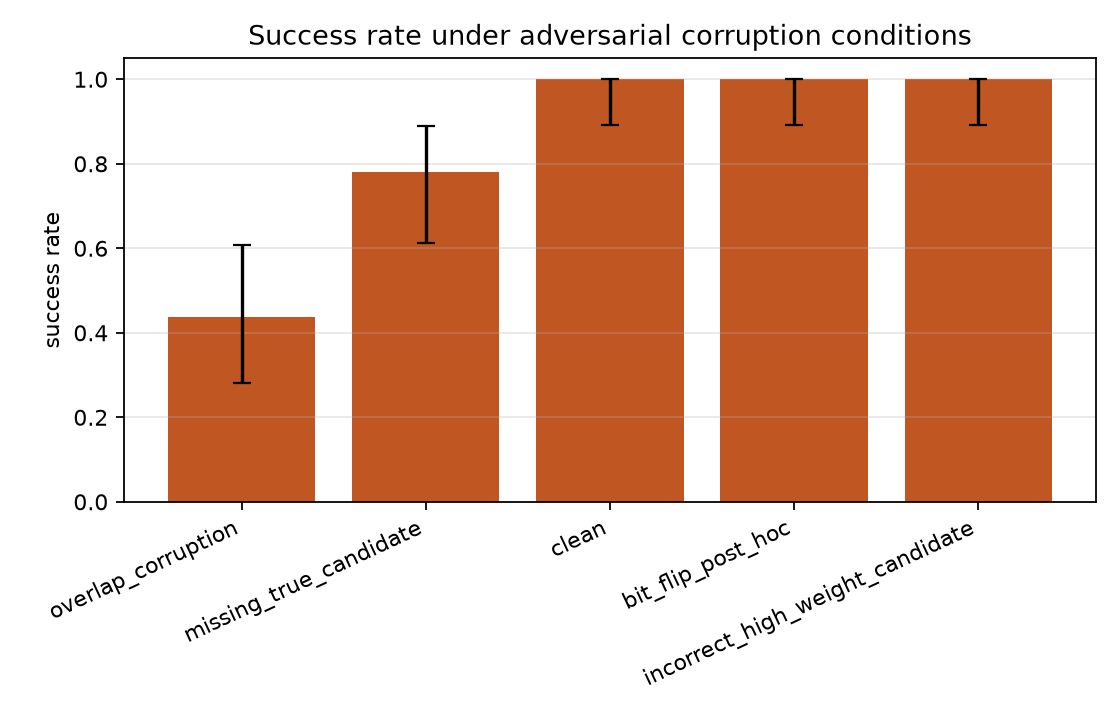
\includegraphics[width=0.78\linewidth]{../Data/failure_study/plots/adversarial_conditions.png}
\caption{\textbf{End-to-end success under direct fault injection}, 32 trials
per condition. The reconstruction logic absorbs post-hoc bit flips and
misleading high-weight candidates completely. Only overlap corruption is
severe, and Sec.~\ref{sec:retraction} shows the mechanism is budget
starvation rather than a defective consistency check. Rendered from
\texttt{phase3\_adversarial.csv}.}
\label{fig:adversarial}
\end{figure}

\subsection{A sharp instability at the ambiguity boundary}
\label{sec:ambiguity}

One failure mode is sharply defined and is not addressed anywhere in this
article. When a window's true phase sits close to the $0.5$ boundary between
adjacent buckets, the winning bit pattern is unstable across repeated
identical measurements. Table~\ref{tab:ambiguity} locates the transition
precisely: at distance $\delta\le0.005$ from the boundary the winner
disagrees across repeats on \textbf{every} trial, and by $\delta=0.010$ it
disagrees on none.

This is a property of the window geometry, not of the reconstruction budget.
No amount of additional sampling or candidate retention fixes it, because
the two competing patterns are genuinely near-equiprobable. Fixing it
requires revising the window boundaries, which regenerates circuits --- and
is therefore out of scope for a classical post-processing intervention.

\begin{table}[htbp]
\centering\small
\caption{Instability at the bucket boundary, 20 repeated identical
measurements per distance. ``Flagged'' is the fraction a $0.9$ top-share
threshold marks ambiguous; ``winner disagrees'' is the fraction where
repeated identical measurements do not agree on the winning pattern. The
transition is complete within one percentage point of the boundary. From
\texttt{phase3\_ambiguity\_boundary.csv}.}
\label{tab:ambiguity}
\begin{tabular}{@{}lrrrr@{}}
\toprule
$\delta$ from boundary & Top-1 share & 2nd share & Flagged & Winner disagrees \\
\midrule
0.000 & 0.413 & 0.402 & 1.00 & \textbf{1.00} \\
0.001 & 0.412 & 0.401 & 1.00 & \textbf{1.00} \\
0.002 & 0.415 & 0.400 & 1.00 & \textbf{1.00} \\
0.005 & 0.414 & 0.400 & 1.00 & \textbf{1.00} \\
0.010 & 0.423 & 0.391 & 0.80 & 0.00 \\
0.020 & 0.438 & 0.375 & 0.00 & 0.00 \\
0.050 & 0.490 & 0.326 & 0.00 & 0.00 \\
0.100 & 0.571 & 0.255 & 0.00 & 0.00 \\
0.250 & 0.811 & 0.091 & 0.00 & 0.00 \\
\bottomrule
\end{tabular}
\end{table}

\section{Scaling, and a compilation cliff that bounds everything}
\label{sec:cliff}

The windowed formulation's central claim is that phase-register width
decouples from precision, and our measurements confirm it: window count and
per-circuit qubit width stay flat as precision rises
(Fig.~\ref{fig:scaling}).

\textbf{The binding constraint is elsewhere, and it is severe.} The
modular-arithmetic work register does not decouple, and in our reference
implementation it is compiled as a dense unitary. Table~\ref{tab:cliff}
gives the measured transpilation time: $0.14$\,s at 4 work qubits,
$0.38$\,s at 5, $2.1$\,s at 6, $42.2$\,s at 7, and a timeout at 8
($N\approx143$). The cliff is in Qiskit's generic unitary synthesis, not in
simulation, and it bites \emph{before a single shot is sampled}.

Two consequences follow, and they constrain every number in this article and
its companion. First, the reachable corpus is $N\le119$ in principle and
$N\in\{15,21\}$ in practice, since within the ceiling only those admit an odd
two-prime modulus with the even, non-trivial order that factor extraction
requires. Second, this is an artefact of our implementation choice, not of
the windowed method: a reversible ripple-carry construction
\cite{cuccaro2004} would replace the dense unitary and move the cliff. We
did not implement one, and we report the ceiling as an open limitation
rather than a property of the algorithm.

\begin{table}[htbp]
\centering\small
\caption{Measured transpilation time for the modular-multiplication
operator, before any sampling. The rise between 6 and 7 work qubits is a
factor of 20, and 8 work qubits does not complete within a $45$\,s timeout.
This is what confines the study to $N\in\{15,21\}$. From
\texttt{phase4\_transpile\_cliff.csv}.}
\label{tab:cliff}
\begin{tabular}{@{}rrrl@{}}
\toprule
$N$ & Work qubits & Transpile (s) & Status \\
\midrule
15  & 4 & 0.14  & completes \\
21  & 5 & 0.38  & completes \\
33  & 6 & 2.09  & completes \\
65  & 7 & 42.23 & completes \\
143 & 8 & $>45$ & \textbf{timeout} \\
\bottomrule
\end{tabular}
\end{table}

\begin{figure}[htbp]
\centering
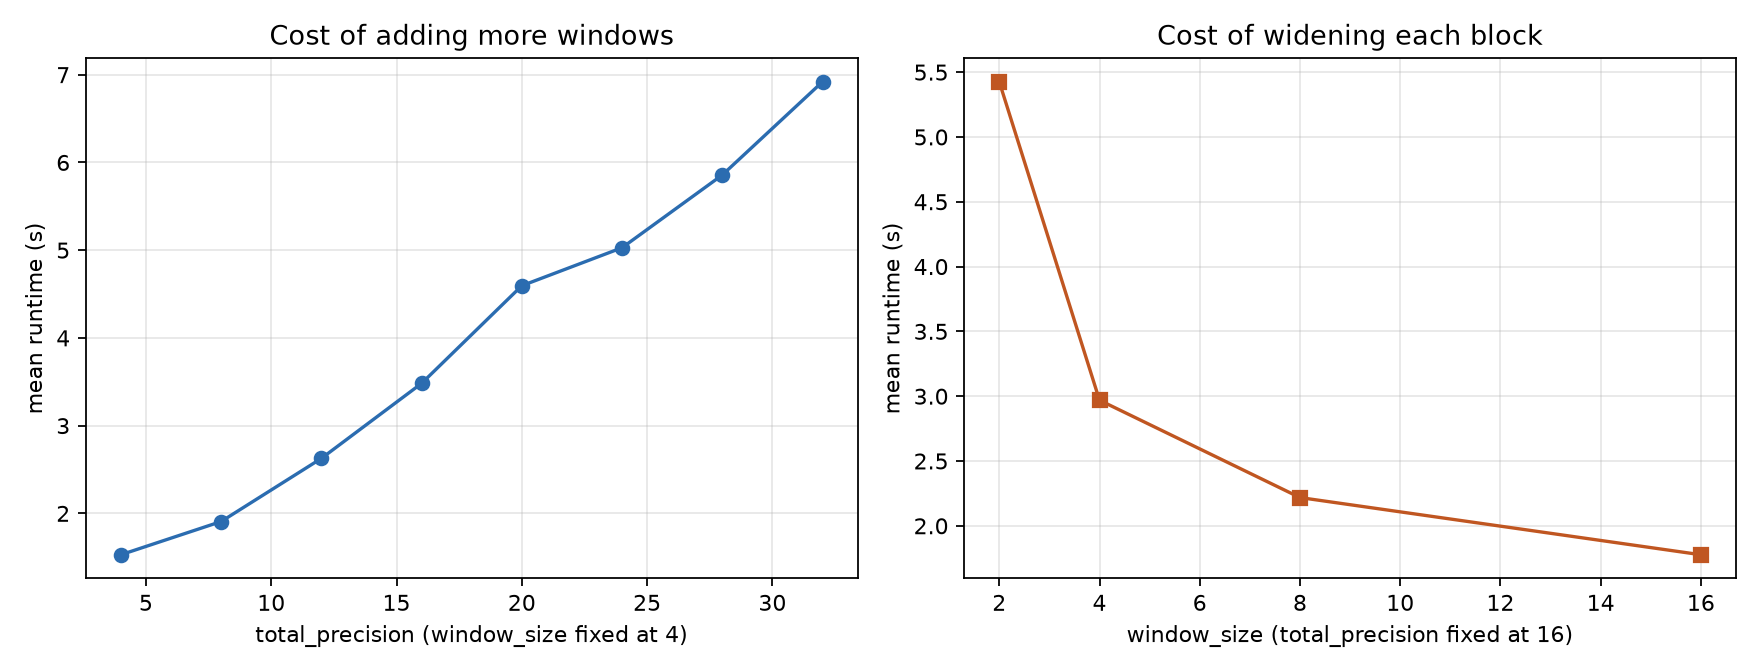
\includegraphics[width=0.86\linewidth]{../Data/failure_study/plots/scaling_decoupling.png}
\caption{\textbf{The decoupling claim holds on the phase side.} Window count
and per-circuit width stay flat as requested precision rises, which is the
saving the windowed formulation promises. The constraint that actually
bounds this study is on the work-register side and is in
Table~\ref{tab:cliff}. Rendered from \texttt{phase4\_scaling\_by\_*.csv}.}
\label{fig:scaling}
\end{figure}

% =====================================================================
\section{What actually causes the failures}
\label{sec:attribution}

The preceding sections produce failures; this one attributes them. Every
failure observed anywhere in the campaign --- 94 in total --- was replayed
through a fixed counterfactual ladder, relaxing one confound at a time and
recording the first rung that recovers the trial: exact bits $\to$ widened
beam $\to$ exhaustive candidates $\to$ noise disabled $\to$ ten-fold shots.
Assigning each failure to the first rung that fixes it gives a partition,
not an overlapping set of contributing factors.

\textbf{Sixty-eight of the 94 failures --- $72\%$ --- are attributed to
classical budget starvation}, not to noise, not to corruption, and not to
any defect in the reconstruction logic (Fig.~\ref{fig:pareto}). Of those, 48
are recovered by additional shots alone, and 20 resist every single-axis
relaxation and need candidate budget \emph{and} beam width widened together.
Noise accounts for 25 ($27\%$), and one trial timed out during attribution.

That 20-failure group is the most informative. It is the direct
counterexample to the single-parameter design of Sec.~\ref{sec:ofat}, and it
is why a fix that widens one budget at a time would be insufficient.

\textbf{Scope of this attribution.} These proportions characterise the
corpus we generated, under a grid we chose to make failures observable. They
are not an estimate of the failure distribution of windowed phase estimation
in general, and we do not present them as one. What they support is a
narrower and sufficient claim: within this corpus, the classical
reconstruction stage --- not the circuit, not the noise model --- is where an
intervention should go.

\begin{figure}[htbp]
\centering
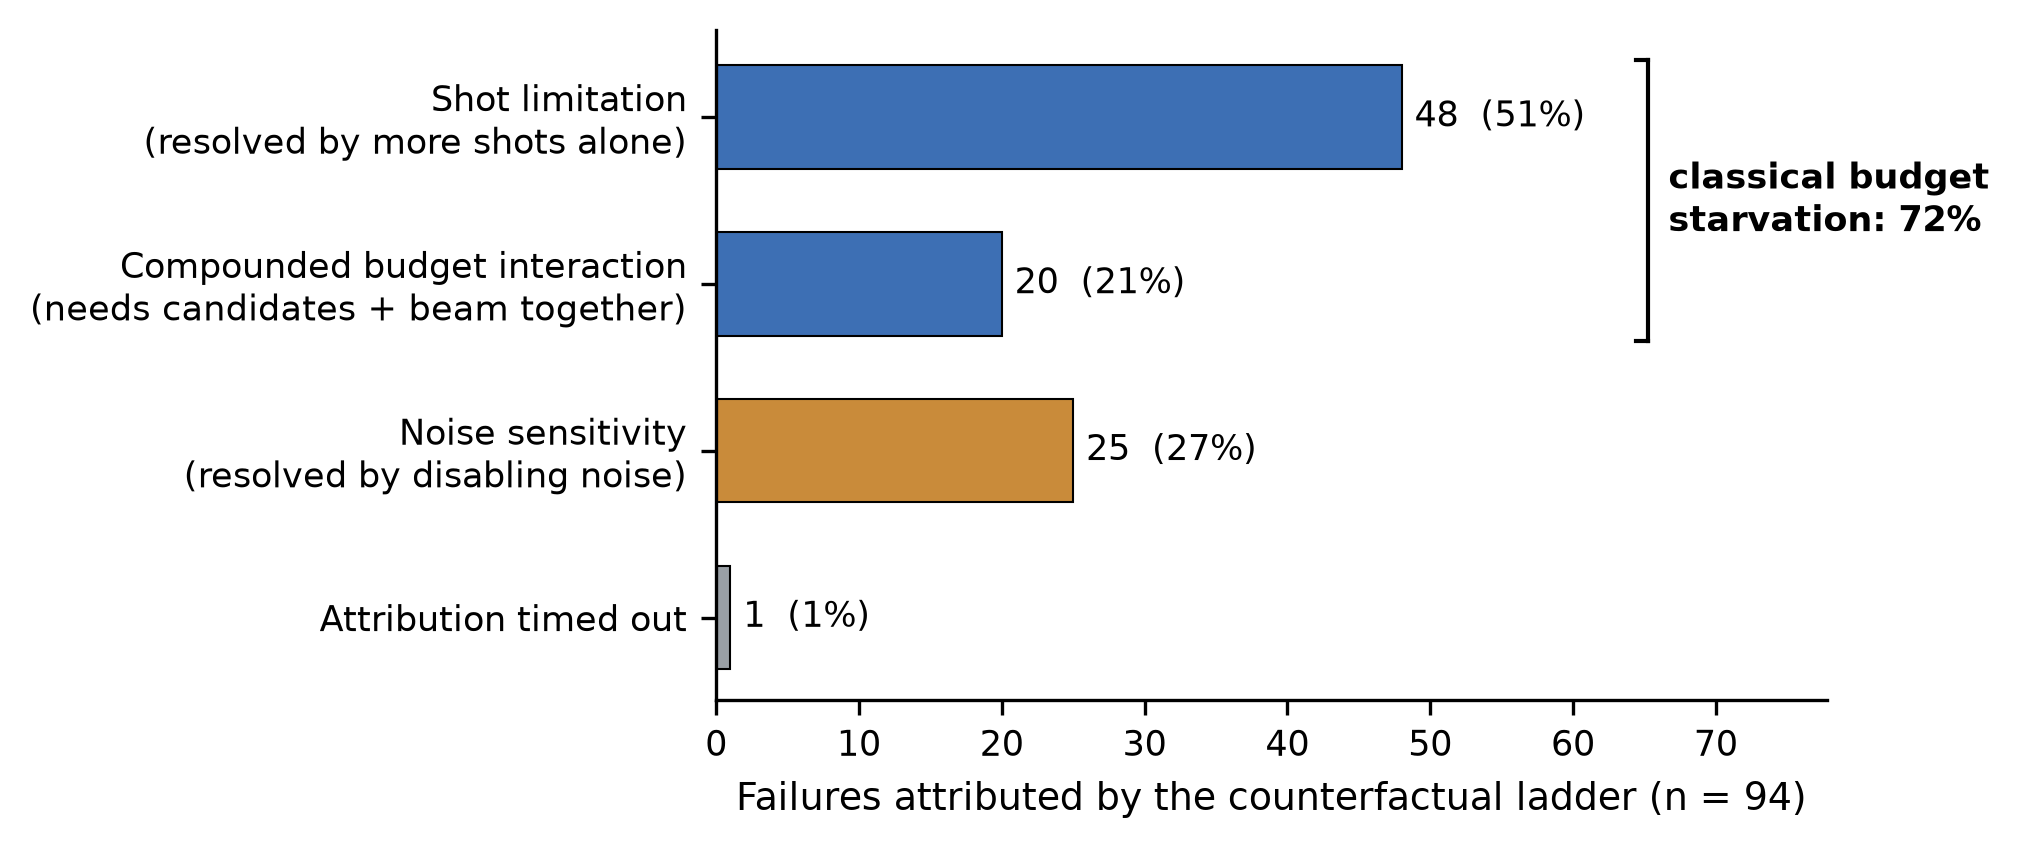
\includegraphics[width=\linewidth]{../Data/failure_study/plots/paper_fig2_failure_attribution.png}
\caption{\textbf{Which mechanism should a fix target?} Root-cause
attribution of all 94 failures observed anywhere in the characterisation
campaign, each replayed through the same counterfactual ladder and
assigned to the first rung that recovers it. Within this corpus the two
classical-budget mechanisms (blue) account for 72\% of failures between
them: 48 that
additional shots alone resolve, and 20 that resist every single-axis
relaxation and need candidate budget and beam width widened together.
Noise (orange) accounts for 27\%. This distribution is what selects the
classical reconstruction stage, rather than the circuit or the noise
model, as the place to intervene. Rendered from
\texttt{phase5\_attribution.csv}.}
\label{fig:pareto}
\end{figure}

% =====================================================================
\section{An error of our own, and what re-validating it saved}
\label{sec:retraction}

Between the characterisation and the intervention we planned a fourth
module, A, to fix the carry-aware overlap check. Our own Phase 3 audit had
reported that the check false-accepts $55.4\%$ of all possible overlap bit
patterns --- serious over-permissiveness in a mechanism central to the
published method, and consistent with the $43.8\%$ success rate under
overlap corruption in Sec.~\ref{sec:adversarial}.

Re-validating that evidence before writing any code showed the finding was
wrong, and wrong in the audit rather than in the mechanism. \textbf{The audit
script pinned the actual computed overlap to one bit regardless of the
nominal overlap width it was sweeping}, so the overlapping bit strings were
never compared at their declared width. The swept parameter did not vary the
quantity it named.

Three independent checks establish the correction.

\begin{enumerate}\itemsep2pt
\item \emph{Algebraically}, the implementation's acceptance condition and the
audit's ground-truth oracle reduce to the same Boolean function, so the
original test could only ever have detected its own bug. The companion
article~\cite{methodpaper} states and proves this.
\item \emph{Empirically}, the same exhaustive 168-combination audit re-run on
corrected geometry gives \textbf{0\% false-accept and 0\% false-reject}
across all three overlap widths --- 42 true accepts and 126 true rejects,
with no error of either kind (\SIaudit{}).
\item \emph{By instrumented replay}, a deliberately corrupted candidate was
rejected in all 80 trials of the overlap-corruption condition.
\end{enumerate}

Two consequences follow. Module A was deleted from the design before any
code was written, and the carry-check implementation required no change. The
residual failures under overlap corruption are explained by the same
budget-starvation mechanism as everything else in Sec.~\ref{sec:attribution}
--- the corrupted candidate is correctly rejected, and a narrow beam then has
no alternative path left --- rather than by the check being fooled.

We report this at length for two reasons. The corrected result is what
justifies leaving the carry check untouched, so the reader needs it to
evaluate the intervention in Part II. And the failure pattern it exposes ---
a swept parameter that does not in fact vary the quantity it names --- is a
reusable warning for anyone building comparable audits. The prior reports
were corrected in place with visible strikethrough rather than silently
edited.

% =====================================================================
\part*{Part II --- Evaluation}
\addcontentsline{toc}{part}{Part II --- Evaluation}

\section{What is being evaluated}
\label{sec:method}

Part I concluded that the classical reconstruction budget is where an
intervention should go. The intervention evaluated here is
confidence-guided adaptive reconstruction, specified in full in the
companion article~\cite{methodpaper}; this section states only what is
needed to read the results.

A per-window posterior comparison statistic $\Cw$ --- the posterior
probability, under a two-proportion Beta model with Jeffreys priors, that
the most-observed bit pattern's true sampling probability exceeds the
runner-up's --- is computed from counts already measured. It drives three
independently switchable modules, each replacing one of the three fixed
budgets of Sec.~\ref{sec:pipeline}: \textbf{B} retains candidates to a
target probability mass instead of a fixed top-$k$; \textbf{C} scales the
beam width by how many windows needed that expansion; \textbf{D} resamples
windows whose $\Cw$ falls below a threshold, up to a hard cap. With all
three disabled the implementation reduces to the published pipeline, which
Sec.~\ref{sec:baselinecheck} verifies trial by trial.

The quantum circuit, its width, its depth and its sampling procedure are
unchanged. Five arms are compared throughout: Baseline, B, C, D, and Full
(all three enabled).

% =====================================================================
\subsection{Design}
\label{sec:design}

Validation proceeds in three stages, addressing in turn whether the
method works, whether it works on instances it was not designed against,
and whether what works is the adaptivity or merely the extra budget.

\paragraph{Stage 1 --- ablation on the canonical grid.} We reuse the
144-cell combined-stress grid of Sec.~\ref{sec:combined} (72 parameter
combinations $\times$ 2 repeats, $N=21$, $a=19$, $r=6$) and run all five
arms on every cell. Each trial's seed is derived deterministically from
its grid coordinates, so a given cell produces identical sampled counts
under every arm and only the classical stage differs --- the pairing that
makes this a within-subjects design.

\paragraph{Stage 2 --- pre-specified held-out instances.} The grid above
is the one that identified budget starvation as the failure mode, so it
cannot speak to generalisation. We re-ran the identical design, unchanged,
on three instances chosen by a rule fixed before any trial of this stage:
the lowest valid base achieving each target order, excluding the
canonical $a=19$. This gives $(N{=}15,a{=}2,r{=}4)$ --- new modulus and
order; $(N{=}21,a{=}8,r{=}2)$ --- canonical modulus, new order; and
$(N{=}21,a{=}2,r{=}6)$ --- canonical order, new base.

The choice set is small, and we state why rather than presenting it as
preference. Within the ${\le}5$ work-qubit ceiling forced by the
compilation cliff (Sec.~\ref{sec:limitations}, Limitation~1), only
$N\in\{15,21\}$ admits an odd two-prime modulus with an even, non-trivial
order, which factor extraction requires. Since $r=6$ at $N=21$ is already
the largest reachable even order, held-out instances broaden \emph{which}
instance is tested but cannot supply one that is \emph{harder}. They
close the circularity objection --- the method was never tuned on them ---
while only narrowing, not eliminating, the external-validity question.
The selection rule was fixed before any trial of this stage ran and is
documented in the module docstring of the script that ran it. We describe
the instances as \emph{pre-specified}: the rule preceded the data, but
it carries no third-party timestamp, so the reader is being asked to
accept a repository artifact rather than an independent record. We make
no claim to the procedural guarantees of a formal registration.

Before Stage 2 ran, the canonical grid was re-executed with resource
instrumentation attached, gated on reproducing the already-recorded
per-trial outcomes bit-for-bit. It did, on all 144 trials.

\paragraph{Stage 3 --- matched-resource controls.} Each module succeeds
partly because it may spend more than baseline. To separate the
allocation \emph{rule} from the allocation \emph{size}, the instrumented
run records each arm's realised budget per trial --- per-window candidate
counts $m_w$, realised beam width $P'$, final per-window shots $S_w$. For
every trial we then build a control given that same realised budget
\emph{uniformly}, evaluated through the Baseline code path with all three
flags disabled, so no confidence guidance appears anywhere in the
control. The shots-matched control redistributes the total extra shots
evenly across windows; the candidates-matched control uses a fixed
$k=\mathrm{round}(\overline{m_w})$; the beam-matched control uses that
trial's realised $P'$ unconditionally. Only the beam-matched control is
exact; the other two approximate a non-uniform allocation by its mean,
and \SItables{} quantifies the residual and its direction.

These controls are deliberately favourable to the baseline: they receive
a budget that could only be known \emph{after} watching the adaptive rule
choose it. They are oracles, not competitors, and the comparison asks
whether confidence guidance beats an allocator that already knows the
answer it would have given.

\paragraph{All three stages are noiseless.} Every trial reported here was
sampled from an ideal simulator with no noise model. This is deliberate:
budget starvation is the failure mode under test, and injecting noise
would add a second, independently varying source of failure the modules
were not built to address. The cost is that the 27\% of
characterisation-campaign failures attributed to noise
(Fig.~\ref{fig:pareto}) fall outside the evaluated regime, and we make no
claim about behaviour when noise rather than budget is the binding
constraint (Limitation~1).

\paragraph{Outcome.} The primary outcome is binary end-to-end success:
the returned phase estimate yields the true order and a non-trivial
factorisation of $N$. Secondary outcomes (realised candidate count, beam
width, additional shots) are in \SItables{}.

\subsection{Statistical methods}
\label{sec:stats}

Outcomes are paired binary, so we use McNemar's test \cite{mcnemar1947},
which Dietterich \cite{dietterich1998} identifies as the appropriate
choice for algorithms evaluated once per unit. We use the \textbf{exact
two-sided binomial form} throughout rather than the $\chi^2$
approximation, because several comparisons have few discordant pairs ---
the C-vs-baseline contrast has only $b+c=7$. Discordant counts $(b,c)$
accompany every $p$-value, since the test is a statement about those
counts alone. Effect sizes are absolute percentage-point differences with
95\% percentile bootstrap intervals, $B=2000$ resamples at fixed seed 0,
resampling the \emph{per-pair differences} so the pairing is preserved
\cite{efron1993}.

We pre-declare \textbf{Full vs.\ Baseline} as the primary comparison. The
confirmatory family comprises the four arm-vs-baseline tests on the
canonical grid, the planned B-vs-C contrast, and the four
adaptive-arm-vs-matched-control tests --- a family of nine, to which
Holm's sequentially rejective procedure \cite{holm1979} is applied
(\SItables{}). The held-out instances are analysed identically
but are \emph{not} pooled into the family: they are replications of an
already pre-declared comparison rather than new hypotheses, so their
$p$-values are reported uncorrected. Full procedural detail is in
\SItables{}.

One consequence deserves flagging here rather than in a footnote:
\textbf{module C's improvement over baseline does not survive the
correction} at this family size ($p=1.6\times10^{-2}$ against a threshold
of $1.25\times10^{-2}$). A smaller five-comparison family covering the
canonical ablation alone would have retained it. We report the larger
family because it is the one the completed validation actually tests.

Following Dietterich, McNemar's test speaks to the difference in error
proportion on \emph{one} evaluation set; two repeats per grid cell do not
characterise variability across independent re-runs of the whole
campaign, and no result here should be read as doing so.

\subsection{Ablation results}
\label{sec:results}

\textbf{Enabling all three modules raised end-to-end success from 52.1\%
to 100.0\% --- an absolute gain of $+47.9$ percentage points (95\%
bootstrap CI $[+39.6, +56.3]$), a relative reduction of 100\% of the
baseline failure rate, on the 144-cell combined-stress grid at $N=21$,
$a=19$, $r=6$.} All 69 baseline failures were converted, and no trial
regressed ($b=0$, $c=69$; exact McNemar $p=3.4\times10^{-21}$).

This is a within-regime result and should be read as one: it is the
comparison the ablation was designed to make, and Secs.~\ref{sec:heldout}
and \ref{sec:matched} each qualify it materially.

Per-arm figures for this grid appear as the first block of
Table~\ref{tab:heldout}, alongside the held-out instances, so that the
canonical and replication results can be read against each other rather
than in separate tables. Module B (candidate coverage) and module D (shot
stopping) each recover roughly half the baseline failure rate on their
own, at $+25.0$ and $+24.3$ percentage points. Module C (beam width)
moves the success rate by only $+4.9$ points on seven discordant trials
and does not survive Holm correction at the confirmatory family size
(\SItables{}); it should be read as a null result rather than a
small positive one. The planned B-vs-C contrast confirms the asymmetry:
B outperforms C by $20.1$ points (95\% CI $[+12.5,+29.2]$, $(b,c)=(8,37)$
counting C as the reference, $p=1.5\times10^{-5}$), and the same contrast
reproduces on the held-out $(N{=}21,a{=}2,r{=}6)$ instance at $+21.5$
points ($p=3.1\times10^{-6}$).



\paragraph{The modules are not interchangeable.} B at 77.1\% and C at
56.9\% do not compose to Full's 100\%, consistent with the attribution of
Sec.~\ref{sec:attribution}: 20 of the 69 hardest failures needed candidate
budget \emph{and} beam width relaxed together, and neither axis alone
reaches them. D's effect size closely matching B's likewise corroborates
the shot-limitation attribution (48 of 69) --- a prediction the design
made in advance rather than a post-hoc reading.

\paragraph{Individual modules can regress individual trials.} Module B
turned two baseline successes into failures, and module D six. These are
not measurement noise; they are the expected consequence of a point made
in the companion article~\cite{methodpaper}. Relaxing a budget changes which
candidates are retained and how the resulting paths rank, and the
continued-fraction stage is not monotone in the candidate set --- a
different phase can be tried first and fail where the baseline's would
have succeeded. Both regressions are absorbed in the Full arm, which
regresses no trial on any of the four instances, but a practitioner
enabling B or D \emph{alone} should expect a small rate of such
reversals; on $(N{=}15,a{=}2,r{=}4)$ module D alone breaks exactly as
many trials as it fixes (Sec.~\ref{sec:heldout}). We flag this because
the structural monotonicity result invites the opposite conclusion.

\subsection{Generalisation to held-out instances}
\label{sec:heldout}

The result above was obtained on the grid that motivated the method, so
on its own it establishes only that the fix works where the fault was
found. Stage 2 re-runs the identical design on three instances the
modules were never tuned against, selected by the pre-specified rule of
Sec.~\ref{sec:design}. Table~\ref{tab:heldout} and
Figure~\ref{fig:heldout} give the outcome; all four grids completed
144/144 trials.

\textbf{The canonical effect replicates.} On $(N{=}21,a{=}2,r{=}6)$ ---
same order, base never used in design --- Full raised success from 50.0\%
to 97.9\%, $+47.9$ percentage points ($b{=}0$, $c{=}69$,
$p=3.4\times10^{-21}$), numerically the same gain as on the canonical
instance; B and D reproduce their canonical effects ($+26.4$ and
$+29.2$ pp) and B again beats C ($+21.5$ pp, $p=3.1\times10^{-6}$). This
is the paper's generalisation evidence, and it is why the circularity
objection does not stand. It also lands at \textbf{97.9\%, not 100\%}:
three of 144 trials still fail, so the honest summary of the method's
ceiling on instances with headroom is $97.9$--$100\%$.

\textbf{Where the baseline has no headroom, no module helps or hurts.} On
$(N{=}21,a{=}8,r{=}2)$ the published pipeline already succeeds on every
trial and every arm returns 100\% with zero discordant pairs --- a ceiling
effect, not a null effect. That instance is also the clearest in-corpus
demonstration of the small-order confound: at order two the
continued-fraction stage recovers the order from almost any phase, so
nothing upstream can be observed to matter. On $(N{=}15,a{=}2,r{=}4)$
baseline succeeds 88.9\% of the time, and B and Full close the gap
completely ($+11.1$ pp, $b{=}0$, $c{=}16$, $p=3.1\times10^{-5}$) while C
changes nothing and D nets exactly zero, fixing eight trials and breaking
eight.

\textbf{The two weaker modules show their weakness here.} Module C is
null on two of three held-out instances, and on the third repeats the
marginal $+4.9$ pp that fails Holm correction (\SItables{}).
Module D carries the most two-sided discordant counts anywhere in the
study --- $(6,41)$ canonical, $(8,50)$ on the replication, $(8,8)$ on
$(N{=}15,a{=}2)$ --- because additional shots change which pattern ranks
first, and a changed ranking sometimes sends continued-fraction recovery
down an unsuccessful branch. D's aggregate effect is strongly positive
where headroom exists, but its per-trial variance is real.

\begin{table}[htbp]
\centering\small
\caption{Held-out generalisation: baseline versus the full combination on
all four instances, 144 seed-paired trials each. The three held-out
instances were selected by a rule fixed before any trial of that stage
ran. $b$ = trials the arm broke; $c$ = trials it fixed; $p$ is the exact
two-sided binomial McNemar value, uncorrected (these are replications,
not members of the Holm family, \SItables{}). Per-arm rows for
B, C and D on every instance are in \SItables{}, and are plotted in
Fig.~\ref{fig:heldout}.}
\label{tab:heldout}
\resizebox{\linewidth}{!}{%
\begin{tabular}{@{}lccccc@{}}
\toprule
Instance & Baseline & Full & Diff.\ [95\% CI] & $(b,c)$ & Exact $p$ \\
\midrule
$N{=}21$, $a{=}19$, $r{=}6$ \emph{(canonical)}
 & 52.1\% & \textbf{100.0\%} & $+47.9$ pp $[+39.6,+56.3]$ & $(0,69)$ & $3.4\times10^{-21}$ \\
$N{=}21$, $a{=}2$, $r{=}6$ \emph{(held-out)}
 & 50.0\% & \textbf{97.9\%}  & $+47.9$ pp $[+39.6,+56.3]$ & $(0,69)$ & $3.4\times10^{-21}$ \\
$N{=}15$, $a{=}2$, $r{=}4$ \emph{(held-out)}
 & 88.9\% & \textbf{100.0\%} & $+11.1$ pp $[+6.3,+16.0]$  & $(0,16)$ & $3.1\times10^{-5}$ \\
$N{=}21$, $a{=}8$, $r{=}2$ \emph{(held-out, ceiling)}
 & 100.0\% & 100.0\% & $\phantom{0}+0.0$ pp $[+0.0,+0.0]$ & $(0,0)$ & $1.00$ \\
\bottomrule
\end{tabular}
}
\end{table}

\begin{figure}[htbp]
\centering
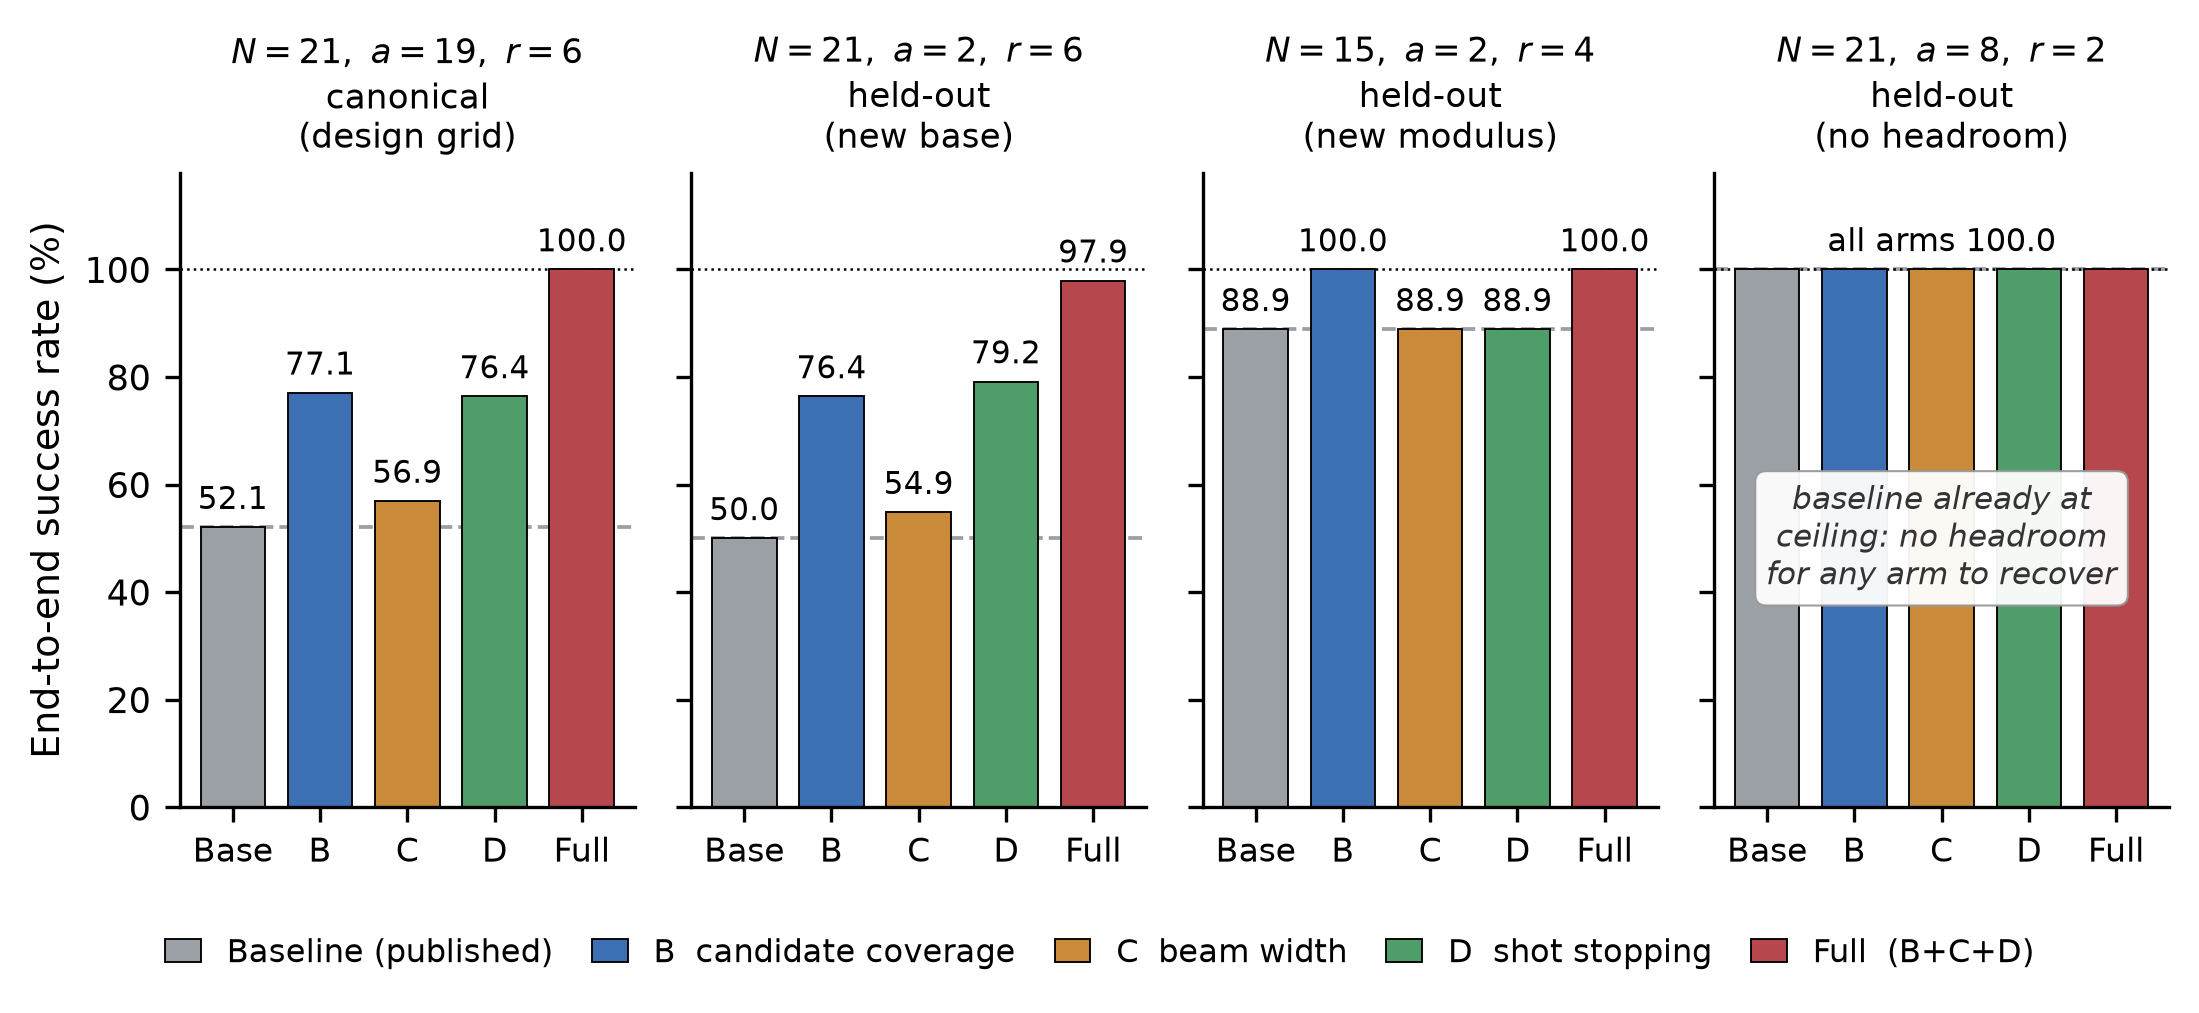
\includegraphics[width=0.94\linewidth]{../Data/failure_study/plots/paper_fig3_heldout.png}
\caption{\textbf{Does the canonical result survive on instances the
modules were never tuned against?} Per-arm end-to-end success on the
canonical instance (left) and the three pre-specified held-out
instances, 144 seed-paired trials each. Dashed line: that panel's
baseline. Dotted line: the 100\% ceiling. The canonical effect replicates
on $(N{=}21,a{=}2,r{=}6)$, a base never used in design, at 97.9\% rather
than 100\%. Headroom shrinks left to right: on $(N{=}15,a{=}2,r{=}4)$
only B and Full move the result, and on $(N{=}21,a{=}8,r{=}2)$ the
published pipeline already succeeds on every trial, so no arm can
demonstrate anything --- a ceiling effect, not a null effect. Module C
changes nothing on either right-hand instance. Rendered from
\texttt{phase6\_ablation\_diagnostics.csv} and
\texttt{phase7\_heldout\_*.csv}.}
\label{fig:heldout}
\end{figure}

\subsection{Matched-resource controls: what is the confidence statistic
actually buying?}
\label{sec:matched}

Every module works by spending more than baseline, which raises the
strongest objection available against this paper and one the ablation of
Sec.~\ref{sec:results} cannot answer: perhaps the gains have nothing to
do with confidence guidance, and any comparable budget increase ---
however allocated --- would do as well. Stage 3 tests exactly this, giving
the Baseline code path each adaptive arm's own realised budget spread
uniformly, with no confidence computation anywhere in the control
(Table~\ref{tab:matched}, Fig.~\ref{fig:matched}).

\textbf{No individual module is distinguishable from its matched
control.} Module B and its candidates-matched control both succeed on
77.1\% of trials, differing on two trials in opposite directions
($b{=}1$, $c{=}1$, $p=1.00$). Module C and its beam-matched control agree
on every single trial ($b{=}c{=}0$, $p=1.00$). Module D reaches 76.4\%
against its control's 73.6\% --- $+2.8$ pp with an interval spanning zero
($[-6.9,+11.8]$, $b{=}22$, $c{=}26$, $p=0.67$), 48 discordant trials
split almost evenly. None comes close to surviving Holm correction
(\SItables{}).

\textbf{The combination is distinguishable.} Full reaches 100\% against
the shots-matched control's 73.6\%: $+26.4$ pp (95\% CI $[+19.4,+33.3]$),
fixing 38 trials the control failed and breaking none ($b{=}0$, $c{=}38$,
$p=7.3\times10^{-12}$). This is the weaker of the two directions the
comparison could have been run in, since the control was matched on shots
alone while Full also widened candidates and beam --- a caveat we return
to below.

\paragraph{What this licenses us to claim, and what it does not.} It does
not license the claim that placing budget by confidence beats placing the
same budget uniformly: at the instance sizes we can reach it does not,
and we found no evidence that it does. What the controls establish is
narrower --- the statistic \emph{recovers} a budget as good as an
oracle-matched uniform one \emph{without being told what that budget
is}. The controls are not algorithms anyone could run: each is built from
diagnostics recorded while watching the adaptive rule make its choices on
that very trial. Sec.~\ref{sec:discussion} develops what this does and
does not support.

There is a second, quantitative reading. The budgets the controls were
handed are large --- a mean of $43.7$ extra shots per window on a grid
whose starved settings are 4--16, a matched candidate count of $4.29$
against a baseline $k\in\{1,2\}$, a matched beam width of $21.1$ against
$P\in\{1,2\}$ (\SItables{}) --- and the adaptive rules arrived at these
multiples from the counts alone. That the uniform version of the same
total performs equally well is a statement about \emph{this} regime: few
windows, small orders, and ambiguity spread fairly evenly across windows.
We would expect the two to separate where ambiguity is concentrated in a
minority of windows, but we have no instance in reach that exhibits that
concentration, so we do not claim it.

\paragraph{How exact is the matching?} The beam-matched control is
exact: $P'$ is already a trial-level scalar, and the control receives
that trial's value unchanged, so its realised beam width equals module
C's on every trial. The other two approximate a non-uniform per-window
allocation by its mean, and the direction of the residual error matters,
so we report it. The candidates-matched control received a mean
$k=4.29$ against module B's mean realised $m_w=4.25$: it was, if
anything, \emph{over}-matched, which makes B's null result harder rather
than easier to obtain. The shots-matched control received a mean of
$43.70$ extra shots per window against the $43.82$ module D actually
drew --- under-matched by $0.3\%$, a shortfall far too small to account
for D's $+2.8$~pp point estimate, and in the direction that favours D.
Neither residual changes the conclusion.

\paragraph{The remaining limit of the controls.} Matching a non-uniform
allocation by its mean is the natural uniform counterpart, but it is not
the only possible one, and a differently-constructed control could
behave differently. More importantly, \textbf{no control matches all
three budgets simultaneously against the Full arm}. The
Full-vs-control comparison equalises shots only, so its $+26.4$~pp
cannot be attributed to confidence guidance alone --- part of it is
simply the candidate and beam budget that the control never received.
Constructing a fully matched three-way control is a direct extension of
the released instrumentation and is the single experiment we would add
next; we flag its absence rather than let the $p=7.3\times10^{-12}$
stand unqualified.

\begin{table}[htbp]
\centering\small
\caption{Matched-resource controls on the canonical 144-trial grid. Each
control runs the Baseline code path, with all module flags disabled, at
the uniform budget derived from that trial's own adaptive diagnostics.
$b$ = trials where the control succeeded and the adaptive arm failed;
$c$ = the reverse. The upper block is the reference gain over an
unmodified baseline; the lower block is the comparison that matters.}
\label{tab:matched}
\resizebox{\linewidth}{!}{%
\begin{tabular}{@{}lccccc@{}}
\toprule
Comparison & Reference & Arm & Diff.\ [95\% CI] & $(b,c)$ & Exact $p$ \\
\midrule
\multicolumn{6}{@{}l}{\emph{Controls do improve on an unmodified baseline}}\\
candidates-matched vs.\ Baseline & 52.1\% & 77.1\% & $+25.0$ pp $[+18.1,+33.3]$ & $(2,38)$ & $1.5\times10^{-9}$ \\
beam-matched vs.\ Baseline       & 52.1\% & 56.9\% & $\phantom{0}+4.9$ pp $[+1.4,+8.3]$ & $(0,7)$ & $1.6\times10^{-2}$ \\
shots-matched vs.\ Baseline      & 52.1\% & 73.6\% & $+21.5$ pp $[+11.8,+31.3]$ & $(13,44)$ & $4.7\times10^{-5}$ \\
\midrule
\multicolumn{6}{@{}l}{\emph{Adaptive arm vs.\ its own matched control}}\\
B vs.\ candidates-matched & 77.1\% & 77.1\% & $\phantom{0}+0.0$ pp $[-2.1,+2.1]$ & $(1,1)$ & $1.00$ \\
C vs.\ beam-matched       & 56.9\% & 56.9\% & $\phantom{0}+0.0$ pp $[+0.0,+0.0]$ & $(0,0)$ & $1.00$ \\
D vs.\ shots-matched      & 73.6\% & 76.4\% & $\phantom{0}+2.8$ pp $[-6.9,+11.8]$ & $(22,26)$ & $0.67$ \\
\textbf{Full vs.\ shots-matched} & \textbf{73.6\%} & \textbf{100.0\%} & $\mathbf{+26.4}$ \textbf{pp} $[+19.4,+33.3]$ & $(0,38)$ & $7.3\times10^{-12}$ \\
\bottomrule
\end{tabular}
}
\end{table}

\begin{figure}[htbp]
\centering
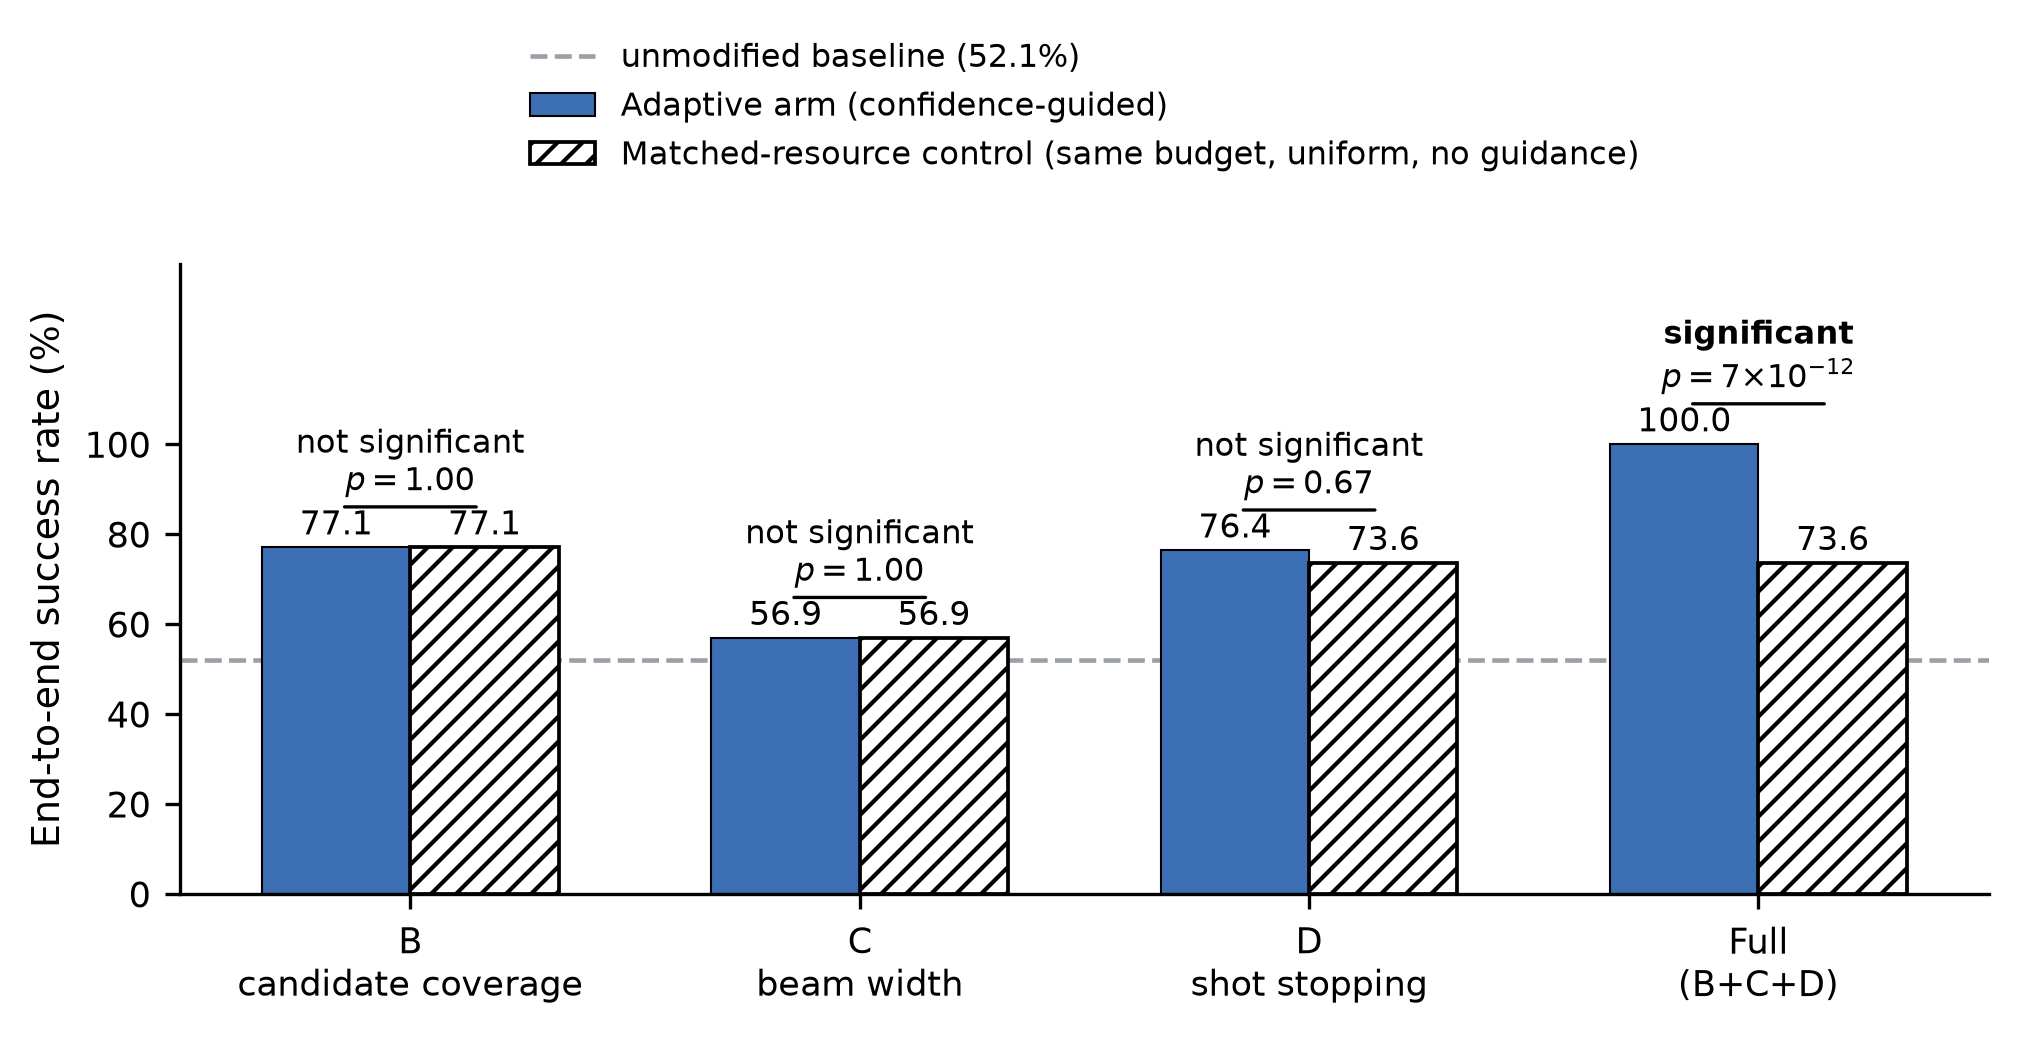
\includegraphics[width=0.94\linewidth]{../Data/failure_study/plots/paper_fig4_matched_resource.png}
\caption{\textbf{Is the gain due to confidence guidance, or to the size
of the budget it requests?} Each adaptive arm beside a control run
through the baseline code path at that arm's \emph{own} realised budget,
spread uniformly, with no confidence computation anywhere. Canonical
grid, 144 seed-paired trials. \textbf{The central result is the three
``not significant'' labels}: taken one at a time, none of the modules
outperforms an equally-resourced uniform allocation. Only the full
combination separates from its control, and that control is matched on
shots alone (Limitation~2). The controls are oracles,
not competitors --- their budgets could only be known after watching the
adaptive rule choose them. Rendered from
\texttt{phase7\_matched\_resource.csv}.}
\label{fig:matched}
\end{figure}


\subsection{Baseline reproduction as a validity check}
\label{sec:baselinecheck}

The companion article's equivalence invariant~\cite{methodpaper} asserts
that the framework with all modules disabled \emph{is} the published
pipeline. That is a claim about code
structure, so measurement cannot establish it --- but measurement can
falsify it, and we checked two ways.

The Baseline arm's success rate reproduces the original combined-stress
figure across three measurements: 52.1\% in the original failure-mode
campaign, 52.1\% in the ablation reported here, and 51.1\% in an interim
run at 139 of 144 trials.\footnote{The interim analysis predates the five
heaviest configurations finishing. The full 144-trial results reported
throughout supersede it; conclusions are unchanged.} The first is not a
re-run of the same function: the original campaign drove the published
pipeline through its own entry point, whereas the Baseline arm is the
adaptive entry point with all flags disabled. Their agreement is
therefore evidence \emph{across} implementations, which a single-function
re-run could not provide.

The second check is stronger than agreement between rates. The
instrumented re-run of Sec.~\ref{sec:design} was gated on reproducing the
recorded per-trial outcomes of \emph{every} arm exactly --- trial by
trial, not in aggregate --- and did so on all 144 trials in all five arms.
Adding the instrumentation that Sec.~\ref{sec:matched} depends on
therefore changed no result, and the seed-paired determinism the whole
design rests on holds in practice rather than merely in principle. Had it
not, the matched-resource controls would have been uninterpretable, since
each is built from a diagnostic recorded during that run.

\subsection{Discussion}
\label{sec:discussion}

\textbf{The central result of this study is not that confidence-guided
allocation has been shown to outperform an equal uniform allocation of
the same total resources.} The matched-resource controls do not support
that claim. What the evidence shows is that the proposed rules can infer
and deploy a workable reconstruction budget from the observed measurement
data, whereas the original pipeline requires that budget to be selected
manually in advance. Every statement elsewhere in this article is scoped
to that reading.

Three findings sit uneasily together at first reading: the combination
of all three modules removes essentially every failure in the regime
where failures occur; individually, no module beats a budget-matched
control; and those controls are themselves not implementable, since they
require knowing in advance what the adaptive rule would have chosen. The
reconciliation is that the modules are not competing with a well-chosen
fixed budget --- they are competing with the problem of choosing one.
Secs.~\ref{sec:ofat} and~\ref{sec:combined} showed that no single starved
budget causes failure while three starved together cause it half the time, so a
practitioner cannot diagnose which knob to turn from a failure alone, and
the correct setting varies cell by cell. That the rule's allocation
performs like an oracle-matched uniform one is the strongest available
evidence that it picks sensible values.

Table~\ref{tab:adopt} states what we would recommend a practitioner
adopt, and on what evidence. The modules are \emph{not} equally
supported, and presenting them as a uniform package would misrepresent
the study.

\begin{table}[htbp]
\centering\small
\caption{Adoption guidance. ``Evidence'' summarises
Secs.~\ref{sec:results}--\ref{sec:matched}; costs are from the companion
article~\cite{methodpaper}.}
\label{tab:adopt}
\begin{tabular}{@{}lp{0.36\linewidth}p{0.36\linewidth}@{}}
\toprule
Module & Evidence & Recommendation \\
\midrule
\textbf{B} coverage
 & Largest and most stable effect; improved every instance with
   headroom; broke at most two trials anywhere.
 & \textbf{Adopt first.} Cheapest of the three: no additional circuit
   execution, same asymptotic class as the code it replaces. \\[3pt]
\textbf{D} shot stopping
 & Large where shots bind, nil where they do not; the most two-sided
   per-trial behaviour in the study.
 & Adopt where sampling is cheap relative to a failed run; it dominates
   wall-clock cost whenever it fires. \\[3pt]
\textbf{C} beam width
 & Fails Holm correction; null on two of three held-out instances;
   indistinguishable from its matched control on every trial.
 & \textbf{Do not enable alone.} Retained in the Full configuration only
   because it provably never narrows the beam and 20 attributed failures
   needed both budget axes relaxed together. \\
\bottomrule
\end{tabular}
\end{table}

None of this is in tension with the calibration result reported in the
companion article~\cite{methodpaper}: module D's stopping rule needs
$\Cw$ to order windows correctly, not to state a correct probability. Where the
miscalibration does cost something is the choice of $\varepsilon$, which
consequently has no principled setting and was left at its default.

% =====================================================================

% =====================================================================
\section{Limitations}
\label{sec:limitations}

We group these into six, ordered by how much each constrains what a
reader may conclude. Each names what would close it; several cannot be
closed by writing.

\paragraph{1. External validity and evaluation scope.}
Every result is at $N\in\{15,21\}$ with $r\in\{2,4,6\}$, noiseless, and
in simulation. \emph{The instance ceiling is not a choice}: the
modular-arithmetic layer of our reference implementation is a dense
unitary whose compilation time rises from $0.4$\,s at 5 work qubits to
$42$\,s at 7 and exceeds a $45$\,s timeout at 8 ($N\approx143$),
foreclosing larger instances before a shot is sampled; within that
ceiling only $N\in\{15,21\}$ admits an odd two-prime modulus with the
even, non-trivial order factor extraction requires. At these orders the
continued-fraction search is very forgiving, and that forgiveness
confounds \emph{any} claim about classical-stage robustness --- the $r=2$
instance, where the unmodified baseline already succeeds on every trial,
demonstrates it directly. \emph{The noiseless scope is a choice}, made to
isolate the mechanism under test, and it leaves the 27\% of
characterisation-campaign failures attributed to noise outside the
evaluated regime. Modules B and C act only on already-sampled counts, but
module D is more exposed: under a noise floor, additional shots can
sharpen confidence in a wrong pattern while consuming the $\Smax$ budget.
We make no claim about behaviour under noise in either direction.
Simulation-only status further excludes the queueing, calibration-drift
and per-shot cost structures D would meet on hardware. \emph{Closing
these:} a reversible modular-arithmetic circuit \cite{cuccaro2004} for
the ceiling; re-running the existing five-arm grid with the noise models
already in the released code, which needs compute rather than new
method.

\paragraph{2. Attribution of the gain to allocation rather than budget.}
Against matched-resource controls, no individual module is
distinguishable from a control given the same realised budget spread
uniformly (Sec.~\ref{sec:matched}). We therefore do not claim that
per-window placement is intrinsically better; the supported claim is that
the rule recovers an oracle-quality budget without being given one. Three
residual gaps qualify even that. \textbf{No control matches all three
budgets against the Full arm}: the Full-vs-control comparison equalises
shots only, so part of its $+26.4$~pp is candidate and beam budget the
control never received, and the figure cannot be attributed to confidence
guidance alone. The shots- and candidates-matched controls approximate a
non-uniform allocation by its mean; only the beam-matched control is
exact (residuals and their directions are quantified in \SItables{}). And
we have no instance whose ambiguity is concentrated in a minority of
windows --- the regime where we would predict placement to separate from
uniform allocation. \emph{Closing these:} a three-way matched control, a
direct extension of the released instrumentation and the single
experiment we would add next.

\paragraph{3. The confidence model.}
$\Cw$'s independence assumption (A2) is measurably false, and the
calibration study quantifies the cost: raw Brier $0.2239$ against
$0.2500$ for a constant $0.5$ forecast, with the top predicted bin at
$0.96$ predicted against $0.79$ observed. The consequence is that
$\varepsilon$ names an error target but delivers a heuristic threshold on
an uncalibrated statistic; it must be tuned empirically rather than set
from a desired error rate, and any extension consuming $\Cw$ as a
probability would be unsound. The isotonic recalibration is deliberately
not wired into the shipped rule, so that the shipped configuration is the
one that was ablated --- and in any case it was fitted and evaluated
in-sample on the same 2{,}687 observations, so its $0.1988$ bounds what
recalibration could achieve rather than estimating out-of-sample
performance. Separately, $\Cw$ compares only the top two patterns (A3),
so a genuine three-way near-tie is not flagged as low-confidence: a
structural blind spot rather than a tuned trade-off, accepted given
$\ell_w\le6$ throughout our corpus. \emph{Closing these:} a
Dirichlet-joint formulation of the statistic~\cite{methodpaper}; a
held-out calibration split.

\paragraph{4. Module-specific evidence.}
\textbf{Module C is not supported as an independent intervention.} It
fails Holm correction at the confirmatory family size
(\SItables{}), is null on two of three held-out instances, and
agrees with its matched control on every trial. Its rule is also
heuristic: $\mathrm{expanded}$ counts ambiguous windows and is not a
derived sufficient beam width. We recommend against enabling it alone and
retain it in the Full configuration only on the strength of its proven
inability to narrow the beam and the 20 compounded failures that needed
both budget axes relaxed together. \textbf{Module B carries no population
coverage guarantee}: $\dcov$ bounds coverage of the observed sample, not
the probability that the true pattern is retained~\cite{methodpaper}; closing that requires a finite-sample
concentration bound we neither derive nor implement. \textbf{Per-trial
regressions are real}: enabled alone, B turned two canonical-grid
successes into failures and D six, and on $(N{=}15,a{=}2)$ D broke
exactly as many trials as it fixed. The Full arm regressed no trial on
any instance, but a practitioner enabling a single module should expect a
small rate of reversals.

\paragraph{5. Parameters and statistical scope.}
$\varepsilon$ and $\dcov$ were used at their published
defaults~\cite{methodpaper} because those defaults already produced large
effects, so no calibration failure prompted a search; we do not know how
sensitive the reported effects are to them, and a looser $\varepsilon$
might capture most of D's benefit at lower sampling cost. The canonical
grid also served both to identify budget starvation and to evaluate the
fix --- the held-out instances of Sec.~\ref{sec:heldout} address that
circularity, but they broaden \emph{which} instance is tested rather than
supplying a harder one. And McNemar's test speaks to one evaluation set:
two repeats per grid cell do not characterise run-to-run variability.

\paragraph{6. Deliberate scope exclusions.}
Window geometry is fixed at configuration time and never revised in
response to confidence (A5), so a separate and sharply-defined failure
mode --- within ${\sim}1\%$ of a window's $0.5$ ambiguity boundary the
winning bucket is unstable across repeated identical measurements --- is
untouched by this framework, which by construction cannot revise geometry
without regenerating circuits. Each window is also allocated
independently, with no shared budget across windows (A4); we did not
analyse jointly constrained allocation because no experiment in our
harness imposes such a budget, which is itself a gap in the evaluation
rather than evidence that coupling would not help.

% =====================================================================
\section*{Ethics statements}
This work involved no human participants, no animal subjects, and no data
collected from social media platforms. All data are generated by numerical
simulation.

\section*{CRediT author statement}
\noindent
Sanjay Lakshmanan R: Conceptualization, Methodology, Software, Validation,
Formal analysis, Investigation, Data curation, Writing -- original draft,
Writing -- review \& editing, Visualization.

\section*{Declaration of competing interest}
The author declares no known competing financial interests or personal
relationships that could have appeared to influence the work reported in
this paper.

\section*{Relation to the companion article}
The method evaluated in Part II is specified in full, with its reusable
adoption protocol, its theoretical properties and its reference
implementation, in a companion article~\cite{methodpaper}. The two articles
share one released corpus and one code archive, and analyse it at different
units: this article at the trial, with end-to-end factorisation success as
the outcome; the companion at the window, against exact per-window
marginals. No figure, table, or result is common to both. In particular, the
per-window records the companion analyses are a re-instrumentation of the
same trials reported in Secs.~\ref{sec:ofat} and~\ref{sec:combined} here.

\section*{Reproducibility}

Every numeric claim in this article is a mechanical summary of a released
result file; \SIartifacts{} maps each file to the script that produced it
and the section that consumes it.

\textbf{Trials are deterministic given their seed.} Each trial's seed is
derived from its grid coordinates and seeds Aer's sampling, so re-running
any cell reproduces its counts exactly. This is what licenses the five-arm
within-subjects comparison, and it was verified rather than assumed: the
instrumented re-run of Sec.~\ref{sec:design} reproduced all 144 canonical
trials, in all five arms, bit-for-bit.

\textbf{The analysis is fully specified}: exact two-sided binomial McNemar;
percentile bootstrap with $B=2000$ resamples at fixed seed 0 over paired
per-trial differences; Holm correction over the family of nine declared in
Sec.~\ref{sec:stats}.

\textbf{Long runs are resumable.} A completed trial is skipped on restart by
its seed, so an interrupted campaign resumes without altering any result ---
necessary in practice, as the heaviest cells take tens of minutes each.

One caveat for anyone recomputing our tables from the released \emph{summary}
CSVs: their two discordant-count columns,
\texttt{baseline\_only\_fixed\_count} and \texttt{arm\_only\_broke\_count},
hold the reverse of what their names suggest --- the first is $b$ (baseline
succeeded, arm failed), the second $c$. The per-trial CSVs are unambiguous
and are what every table here was built from.

\section*{Code availability}
The complete implementation --- quantum circuits, classical reconstruction,
the adaptive modules, and every experiment script named in \SIartifacts{} ---
is released under the Apache-2.0 licence at
\url{https://github.com/Shadow-46/QuantumPhaseReconstruction}. An archived
snapshot will be deposited in a persistent repository and its DOI supplied
at acceptance. Each executable module carries a self-test that runs without
arguments.

\section*{Data availability}
All raw per-trial records, per-window recaptured counts, summary tables, and
figures are released with the code at the same location. No data were
obtained from third parties, and no dataset is under embargo.

\section*{Supplementary material}
A Supplementary Information document accompanies this article, containing
the full carry-audit record, the complete failure-attribution breakdown, the
extended statistical and resource tables, and the artifact map. The
mathematical derivations of the method's properties accompany the companion
article~\cite{methodpaper} instead.

% =====================================================================
\bibliographystyle{elsarticle-num}
\bibliography{refs_B}

\end{document}
